\documentclass{article}
\usepackage{tikz, amsmath, amssymb, pgfplots, enumerate, multirow, multicol}
\usetikzlibrary{shapes,arrows,calc, patterns}
\usepgfplotslibrary{fillbetween}
\usepackage[margin=1in]{geometry}

\title{Supply Concepts}
\author{Ryan Safner}
\date{ECON 306}

\begin{document}

\maketitle

\section*{Firm's Constrained Optimization}

\begin{itemize}
	\item The \textbf{Firms (constrained optimization) problem} is:  
	\begin{enumerate}
		\item \textbf{Choose:} \textcolor{blue}{$<$inputs, output$>$}
		\item \textbf{In order to maximize:} \textcolor{green}{$<$profits$>$}
		\item \textbf{Subject to}: \textcolor{red}{$<$technology$>$}
	\end{enumerate}
	\item We break up the firm's problem into two problems: 
	\item The firm's \textbf{cost-minimization problem}:
	\begin{enumerate}
		\item \textbf{Choose:} \textcolor{blue}{$<$inputs$>$}
		\item \textbf{In order to minimize:} \textcolor{green}{$<$total cost$>$}
		\item \textbf{Subject to}: \textcolor{red}{$<$producing optimal output$>$}
	\end{enumerate}
	\item The firm's \textbf{profit-maximization problem}:
	\begin{enumerate}
		\item \textbf{Choose:} \textcolor{blue}{$<$output$>$}
		\item \textbf{In order to maximize:} \textcolor{green}{$<$profit$>$}
	\end{enumerate}
\end{itemize}

\subsection*{Production \& Firms}
\begin{itemize}
	\item Firms organize production by buying or renting inputs (``factors of production'') and transforming them into outputs according to their \textbf{technology} or \textbf{production function} 
	\begin{equation*}
	q=f(k,l)	
	\end{equation*}
	where $q$ = amount of output, $k$ = amount of capital, and $l$ = amount of labor
	\item Two time-frames of production: 
	\begin{itemize}
		\item \textbf{Short-run}: at least one factor of production is fixed (e.g. $\bar{k}$)
		\begin{itemize}
			\item We can characterize the short-run production function by plugging in the amount of our fixed factor, e.g. 
			\begin{align*}
				q(l,k)&=lk\\
				\bar{k}&=10\\
				q(l,\bar{k})&=10l\\
			\end{align*}
			\item The \textbf{marginal product} of an input measures how output changes as one input is added (holding the other(s) constant): 
			\begin{align*}
			MP_l&=\frac{\Delta q}{\Delta l}\\
			MP_k&=\frac{\Delta q}{\Delta k}\\ 	
			\end{align*}
			\begin{itemize}
				\item Inputs are often assumed to have \textbf{diminishing returns}: $MP$ is declining ($q$ is increasing at a decreasing rate with respect to each input)
			\end{itemize}
		\item The \textbf{average product} of an input measures output per unit of input
		\begin{align*}
		AP_l&=\frac{q}{l}\\
		AP_k&=\frac{q}{k}\\	
		\end{align*}
		
		\begin{table}
		\centering 
		\begin{tabular}{cc}
	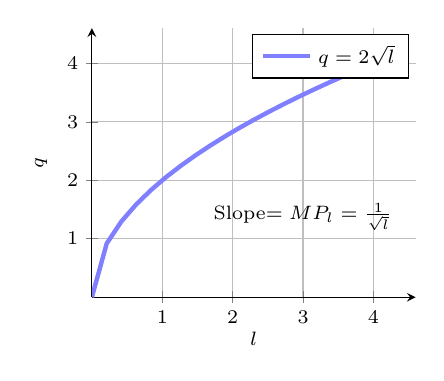
\begin{tikzpicture}\scriptsize 
	\begin{axis}[
		scale=0.6,
		axis lines=middle, 
		enlarge x limits={rel=0.15, upper},
		enlarge y limits={rel=0.15, upper},
		every axis y label/.style={at={(axis description cs:-0.2,0.5)},rotate=90,anchor=north},
		every axis x label/.style={at={(axis description cs:0.5,-0.1)},anchor=north},
	%legend style={at={(0.5,-0.25)},anchor=north},
	xlabel=$l$,
	ylabel=$q$,
	shader=flat,
	xtick={0,1,...,4},
	ytick={0,1,...,4},
	grid=major,
	ymax=4
]
	\addplot[domain=0:4, samples=20, ultra thick, color=blue!50]{2*sqrt(x)};
	\addlegendentry{$q=2\sqrt{l}$};
	\draw[] (axis cs:3,1)node[above]{Slope$=MP_l=\frac{1}{\sqrt{l}}$};
\end{axis}
\end{tikzpicture}
&
	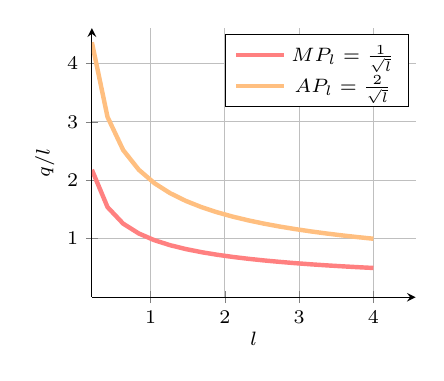
\begin{tikzpicture}\scriptsize 
	\begin{axis}[
		scale=0.6,
		axis lines=middle, 
		enlarge x limits={rel=0.15, upper},
		enlarge y limits={rel=0.15, upper},
		every axis y label/.style={at={(axis description cs:-0.2,0.5)},rotate=90,anchor=north},
		every axis x label/.style={at={(axis description cs:0.5,-0.1)},anchor=north},
	%legend style={at={(0.5,-0.25)},anchor=north},
	xlabel=$l$,
	ylabel=$q/l$,
	shader=flat,
	xtick={0,1,...,4},
	ytick={0,1,...,4},
	grid=major,
	ymax=4,
	ymin=0,
]
	\addplot[domain=0:4, samples=20, ultra thick, color=red!50]{1/sqrt(x)};
	\addlegendentry{$MP_l=\frac{1}{\sqrt{l}}$};
	\addplot[domain=0:4, samples=20, ultra thick, color=orange!50]{2/sqrt(x)};
	\addlegendentry{$AP_l=\frac{2}{\sqrt{l}}$};
\end{axis}
\end{tikzpicture}
		\end{tabular}
		\caption{Short-run production function with diminishing returns}
		\end{table}
		\end{itemize}
		\item \textbf{Long-run}: all factors are variable 
	\end{itemize}
\end{itemize} 

\subsection*{Isocost Lines} 

\begin{itemize}
	\item \textbf{Isocost line}: the combinations of inputs that are the same total cost 
	\begin{equation*}
	wl+rk=C 	
	\end{equation*}
	$w=$ price of labor, $r=$ price of capital
	\begin{itemize}
		\item To graph, solve for $k$: 
		\begin{equation*}
			k=\frac{C}{r}-\frac{w}{r}l
		\end{equation*}
		\clearpage 
		\begin{itemize}
		\item Vertical intercept: $\displaystyle \frac{C}{r}$
		\item Horizontal intercept: $\displaystyle \frac{C}{w}$
		\item Slope: $\displaystyle -\frac{w}{r}$
		\end{itemize}
	\end{itemize} 
	\begin{figure}[h!]
		\centering 
			\begin{tikzpicture}[scale=.4]
			\draw[->] (0,0) -- (11,0) coordinate (x axis) node[right]{$l$};
 			\draw[->] (0,0) -- (0,11) coordinate (y axis) node[above]{$k$};
 			\draw[black, fill=black] (0,5)circle(0.125cm)node[left]{$\frac{C}{r}$};
 			\draw[black, fill=black] (10,0)circle(0.125cm)node[below]{$\frac{C}{w}$};
			\draw[ultra thick, blue] (0,5)--node[above=.25cm]{\textcolor{black}{$k=\frac{C}{r}-\frac{w}{r}x$}}(10,0);
 		\end{tikzpicture}
	\caption{The Isocost Line}
	\end{figure} 
	\item All points on the line are same total cost
	\begin{itemize}
		\item All points beneath line are lower total cost
		\item All points above the line are higher total cost	
	\end{itemize}
	\item Change in an input's market price: rotates isocost line 
		\begin{itemize}
			\item New intercept for input that changed in price
			\item New slope 
		\end{itemize}
	\item Slope of isocost line measures the \emph{market} exchange rate between $l$ and $k$ (their relative prices)
\end{itemize}

\begin{table}[h!]
		\centering 
		\begin{tabular}{cc}
$\Delta w$ ($\uparrow$ in red, $\downarrow$ in green) & $\Delta r$ ($\uparrow$ in red, $\downarrow$ in green)\\
	\begin{tikzpicture}[scale=0.7]\small 
			\draw[->] (0,0) -- (6,0) coordinate (x axis) node[right]{$l$};
 			\draw[->] (0,0) -- (0,6) coordinate (y axis) node[above]{$k$};
	\draw[very thick, blue] (0,3)node[left]{$\frac{C}{r}$}--(3,0)node[below]{$\frac{C}{w}$};
	\draw[very thick, red, dashed] (0,3)--(1,0)node[below]{$\frac{C}{w'}$};
	\draw[very thick, green, dashed] (0,3)--(5,0)node[below]{$\frac{C}{w''}$};
\end{tikzpicture}
&
	\begin{tikzpicture}[scale=0.7]\small 
			\draw[->] (0,0) -- (6,0) coordinate (x axis) node[right]{$l$};
 			\draw[->] (0,0) -- (0,6) coordinate (y axis) node[above]{$k$};
	\draw[very thick, blue] (0,3)node[left]{$\frac{C}{r}$}--(3,0)node[below]{$\frac{C}{w}$};
	\draw[very thick, red, dashed] (0,1)node[left]{$\frac{C}{r'}$}--(3,0);
	\draw[very thick, green, dashed] (0,5)node[left]{$\frac{C}{r''}$}--(3,0);
\end{tikzpicture}\\
\end{tabular}
\caption{How the isocost line changes with input prices} 
\end{table}

\clearpage 

\subsection*{Isoquant Curves}
\begin{itemize}
	\item \textbf{Isoquant curves} link all combinations of inputs that produce the same output 
							\begin{figure}[h!]
							\centering 
	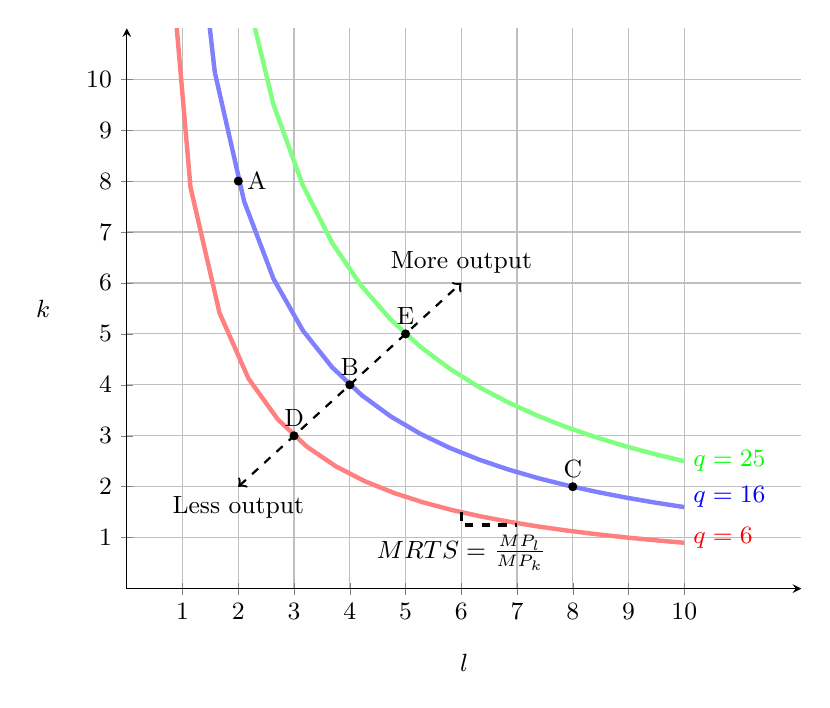
\begin{tikzpicture}\small  
	\begin{axis}[
		scale=1.25,
		axis lines=middle, 
		enlarge x limits={rel=0.1, upper},
		enlarge y limits={rel=0.1, upper},
		every axis x label/.style={at={(axis description cs:0.5,-0.1)},anchor=north},
		every axis y label/.style={at={(axis description cs:-0.1,0.5)},anchor=east},
	%legend pos=outer north east,
	xlabel=$l$,
	ylabel=$k$,
	shader=flat,
	xtick={1, 2,...,10},
	ytick={0,1,2,...,10},
	grid=major,
	ymin=0,
	xmin=0,
	xmax=11,
	ymax=10,
]
	\addplot[name path=ic, domain=0:10, samples=20, ultra thick, color=blue!50]{16/(x)};
	\draw[black, fill=black] (axis cs:2,8)circle(0.05cm)node[right]{A};
	\draw[black, fill=black] (axis cs:8,2)circle(0.05cm)node[above]{C};
	\draw[black, fill=black] (axis cs:4,4)circle(0.05cm)node[above]{B};
	\addplot[domain=0.1:10, samples=20, ultra thick, color=red!50]{9/(x)};
	\draw[black, fill=black] (axis cs:3,3)circle(0.05cm)node[above]{D};
	\addplot[domain=0:10, samples=20, ultra thick, color=green!50]{25/(x)};
	\draw[black, fill=black] (axis cs:5,5)circle(0.05cm)node[above]{E};
	\draw[thick, black, dashed, <->] (axis cs:2,2)node[below]{Less output}--(axis cs:6,6)node[above]{More output};
	\draw[red] (axis cs:10,1)node[right]{$q=6$};
	\draw[blue] (axis cs:10,1.8)node[right]{$q=16$};
	\draw[green] (axis cs:10,2.5)node[right]{$q=25$};
	\draw[very thick, dashed] (axis cs:6,1.5)--(axis cs:6,1.25)node[below]{$MRTS=\frac{MP_l}{MP_k}$}--(axis cs:7,1.25);
\end{axis}
\end{tikzpicture}
\caption{Isoquant curves: $E > A = B = C > D$}
\end{figure}
	\begin{itemize}
	\item \textbf{Marginal rate of technical substitution (MRTS)}: firm's exchange rate between $l$ and $k$
		\begin{itemize}
		\item $MRTS=$ the slope of the isoquant curve
		\item Literally: the amount of $k$ given up to obtain 1 more $k$ produce same output 
		\end{itemize}
	\end{itemize}
 		\begin{itemize}
 			\item Marginal products are related to MRTS: 
 			\begin{equation*}
 			MRTS=\frac{MP_l}{MP_k}	
 			\end{equation*}
	
	\clearpage 
	
	\item Shape \& slopes (MRTS) of isoquant curves:
	\begin{itemize}
	\item Bent vs. straight $\implies$ complementarity vs. substitutability between $l$ and $k$
		\begin{table}[h!]
		\centering 
		\begin{tabular}{cc}
			Right-angle $\implies$ perfect complements & Straight line $\implies$ perfect substitutes\\
			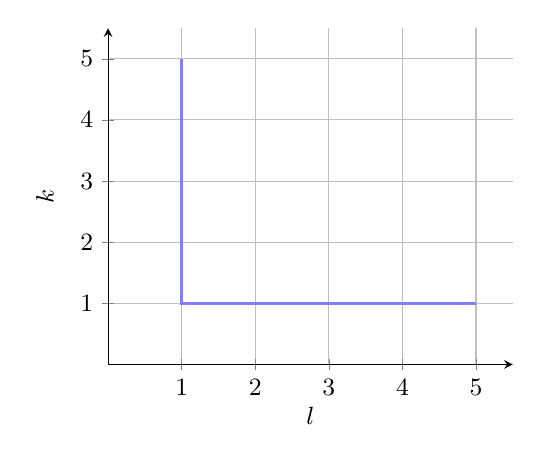
\begin{tikzpicture}\small 
	\begin{axis}[
		scale=0.75,
		axis lines=middle, 
		enlarge x limits={rel=0.1, upper},
		enlarge y limits={rel=0.1, upper},
		every axis y label/.style={at={(axis description cs:-0.2,0.5)},rotate=90,anchor=north},
		every axis x label/.style={at={(axis description cs:0.5,-0.1)},anchor=north},
	%legend pos=outer north east,
	xlabel=$l$,
	ylabel=$k$,
	shader=flat,
	xtick={1, 2,...,5},
	ytick={0,1,...,5},
	grid=major,
	ymin=0,
	xmin=0,
]
	\addplot[opacity=0]{x};
	\draw[very thick, blue!50] (axis cs:1,5)--(axis cs:1,1)--(axis cs:5,1);
\end{axis}
\end{tikzpicture}
&
	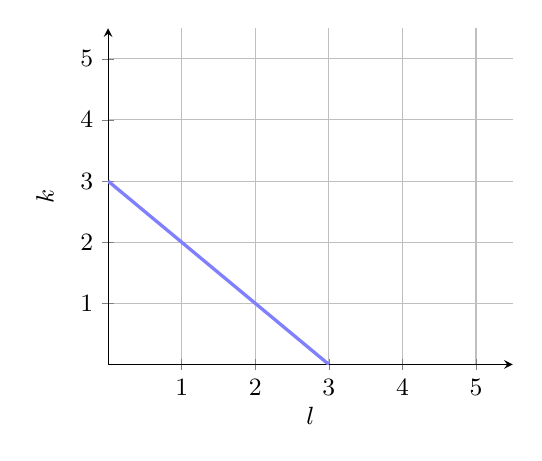
\begin{tikzpicture}\small 
	\begin{axis}[
		scale=0.75,
		axis lines=middle, 
		enlarge x limits={rel=0.1, upper},
		enlarge y limits={rel=0.1, upper},
		every axis y label/.style={at={(axis description cs:-0.2,0.5)},rotate=90,anchor=north},
		every axis x label/.style={at={(axis description cs:0.5,-0.1)},anchor=north},
	%legend pos=outer north east,
	xlabel=$l$,
	ylabel=$k$,
	xtick={1, 2,...,5},
	ytick={0,1,...,5},
	grid=major,
	ymin=0,
	xmin=0,
]
	\addplot[opacity=0]{x};
	\draw[very thick, blue!50] (axis cs:0,3)--(axis cs:3,0);
\end{axis}
\end{tikzpicture}\\
Always produce at same rate of combination & Always substitute at same rate\\
\end{tabular}
\end{table}
	\end{itemize}
\end{itemize}
	\clearpage 

\subsection*{Solving the Firm's Cost-Minimization Problem}

\begin{itemize}
	\item Firm chooses combination of $l$ and $k$ to minimize total cost while producing the optimal amount of output 	
	\begin{itemize}
		\item Expressed mathematically: 
	\begin{equation*}
		\min_{\textcolor{blue}{l,k}} \textcolor{green}{wl+rk}
		\end{equation*}
		\begin{equation*}
		\text{ s. t. }\textcolor{red}{q^*=f(k,l)} 
	\end{equation*}
		\item Graphically: optimum is the point of tangency between the lowest isocost line tangent to the (optimal) isoquant
				\begin{figure}[h!]
		\centering 
			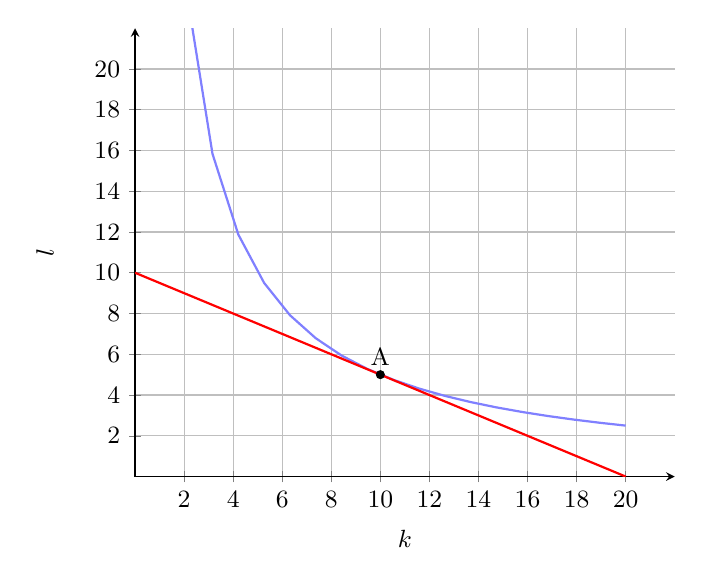
\begin{tikzpicture}\small  
	\begin{axis}[
		scale=1,
		axis lines=middle, 
		enlarge x limits={rel=0.1, upper},
		enlarge y limits={rel=0.1, upper},
		every axis y label/.style={at={(axis description cs:-0.2,0.5)},rotate=90,anchor=north},
		every axis x label/.style={at={(axis description cs:0.5,-0.1)},anchor=north},
	legend style={at={(0.5,-0.25)},anchor=north},
	ylabel=$l$,
	xlabel=$k$,
	xtick={2,4,...,20},
	ytick={0,2,...,20},
	grid=major,
	ymin=0,
	xmin=0,
	ymax=20,
	xmax=20
]
	\addplot[thick, color=blue!50, domain=0:20, samples=20, forget plot]{50/x};
	\draw[thick, red](axis cs:0,10)--(axis cs:20,0);
	\addlegendimage{thick, red};
	\addlegendimage{thick, blue!50};
	\draw[fill=black](axis cs:10,5)circle(0.05cm)node[above]{A};
\end{axis}
\end{tikzpicture}	
\caption{The firm's optimum at point $A$: isoquant curve is tangent to isocost line}
		\end{figure}
		\item At the tangency point ($A$), all of the following are true: 
		\begin{align*}
		|\text{Slope of I.Q. Curve}|	&=|\text{Slope of I.C. Line}| & & \text{Slopes are equal}\\
		MRTS&=\frac{w}{r} & & \text{Definition of each slope}\\
		\frac{MP_l}{MP_k}&=\frac{w}{r} & & \text{Firm's exchange rate same as market exchange rate}\\
		\frac{MP_l}{w}&=\frac{MP_k}{r} & & \text{Marginal product per \$1 is the same between $l$ and $k$}\\
		\end{align*}
		\end{itemize}
	\item \textbf{Equimarginal principle}: output is optimized when firm can lower costs no more output by spending \$1 more/less on either $l$ or $k$
	\begin{itemize}
		\item Firm is indifferent between using more $l$ or using more $k$: has no reason to change input decisions! 
		\item If marginal product per dollar were greater for (e.g.) $l$ than for $k$, could buy more $l$ and lower costs! 
	\end{itemize}
	\end{itemize} 
	\item \textbf{Returns to Scale}: technological relationship between scaling all inputs at the same rate and the scale of output
	\begin{itemize}
		\item Constant returns to scale: output scales at the same rate as scaling all inputs
		\begin{itemize}
			\item e.g. doubling all inputs doubles output
		\end{itemize}
		\item Increasing returns to scale: output scales at a faster rate than scaling all inputs 
		\begin{itemize}
			\item e.g. doubling all inputs more-than-doubles output
		\end{itemize}
		\item Decreasing returns to scale: output scales at a slower rate than scaling all inputs 
		\begin{itemize}
			\item e.g. doubling all inputs less-than-doubles output
		\end{itemize}
\end{itemize}
\end{itemize}

\clearpage 
\section*{Supply in Competitive Markets}

\subsection*{Costs}

\begin{itemize}
	\item Economic vs. accounting concepts: 
	\begin{itemize}
		\item Accounting costs: monetary costs
		\item Economic (opportunity) costs: value of next best opportunity given up 
		\item Accounting profit: Total revenue minus accounting costs
		\item Economic profit: Total revenue minus accounting \& economic costs
		\item Accounting point of view: are you taking in more cash than you are spending
		\item Economic point of view: are you really making the \emph{best} use of your resources with your current project (i.e. is there a higher-value use)? 
		\begin{itemize}
			\item Implications for society: consumers really \emph{best} off with you using scarce resources (with other uses) to produce your current product?
		\end{itemize} 	
	\end{itemize}
	\item Total cost function $C(q)$ relates total quantity of output $q$ (using optimal combinations of $l$ and $k$) to the total cost of production $C$
	\begin{equation*}
	C(q)=FC+VC(q)	
	\end{equation*}
	\begin{itemize}
		\item Fixed Costs $FC$: costs that do not vary with output
		\item Average Fixed Costs $AFC(q)$: fixed costs per unit 
		\begin{equation*}
		AFC(q)=\frac{FC}{q}	
		\end{equation*}
		\item Variable Costs $VC(q)$: costs that vary with output
		\item Average Variable Cost $AVC(q)$: variable cost per unit of output 
		\begin{equation*}
		AVC(q)=\frac{VC}{q}	
		\end{equation*}
		\item Average (Total) Cost $AC(q)$: (total) cost per unit of output 
		\begin{align*}
		AC(q)&=\frac{TC}{q}\\
		AC(q)&=AFC(q)+AVC(q)\\	
		\end{align*}
		\item Marginal Cost ($MC(q)$): how cost changes with one unit of output 
		\begin{equation*}
		MC(q)=\frac{\Delta C(q)}{\Delta q}	
		\end{equation*}
		
		\begin{table}
			\centering 
			\begin{tabular}{cc}
		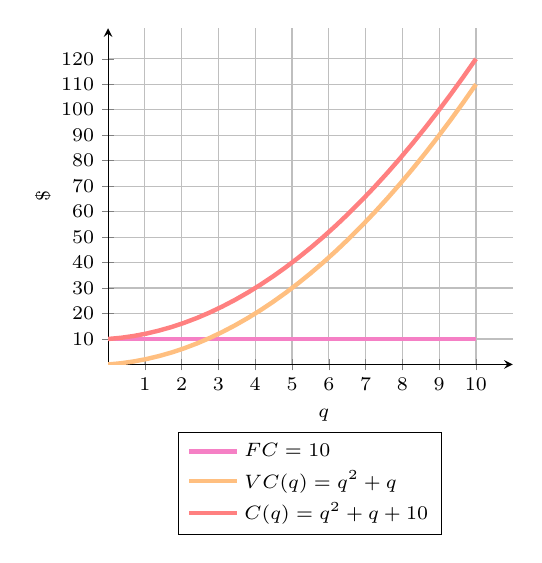
\begin{tikzpicture}\scriptsize
	\begin{axis}[scale=0.75,
		xlabel=$q$,
		ylabel=$\$$,
		grid=major,
		legend style={at={(0.5,-0.2)},anchor=north},
		ymin=0,
		xtick={0,1,...,10},
		ytick={0,10,...,120},
				axis lines=middle, 
		enlarge x limits={rel=0.1, upper},
		enlarge y limits={rel=0.1, upper},
		every axis y label/.style={at={(axis description cs:-0.2,0.5)},rotate=90,anchor=north},
		every axis x label/.style={at={(axis description cs:0.5,-0.15)},anchor=west},
		legend cell align=left,
		ymax=120,
		xmax=10,
		xmin=0]
		\addplot[domain=0:10, opacity=0, forget plot]{x};
		\addplot[ultra thick, domain=0:10,magenta!50, samples=30]{10};
		\addlegendentry{$FC=10$}
		\addplot[ultra thick, domain=0:10,orange!50, samples=30]{x+x^2};
		\addlegendentry{$VC(q)=q^2+q$}
		\addplot[ultra thick, domain=0:10,red!50, samples=30]{x^2+x+10};
		\addlegendentry{$C(q)=q^2+q+10$}
		\end{axis}
 			\end{tikzpicture}
&
			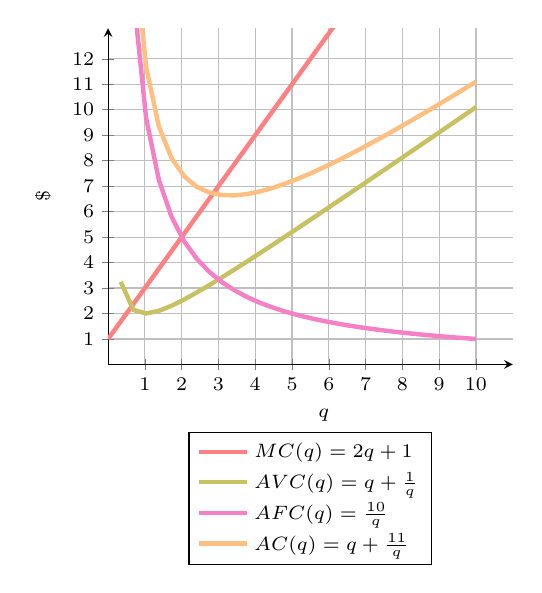
\begin{tikzpicture}\scriptsize
	\begin{axis}[scale=0.75,
		xlabel=$q$,
		ylabel=$\$$,
		grid=major,
		legend style={at={(0.5,-0.2)},anchor=north},
		legend cell align=left,
		ymin=0,
		xtick={0,1,...,10},
		ytick={0,1,...,12},
				axis lines=middle, 
		enlarge x limits={rel=0.1, upper},
		enlarge y limits={rel=0.1, upper},
		every axis y label/.style={at={(axis description cs:-0.2,0.5)},rotate=90,anchor=north},
		every axis x label/.style={at={(axis description cs:0.5,-0.15)},anchor=west},
		ymax=12,
		xmax=10,
		xmin=0]
		\addplot[domain=0:10, opacity=0, forget plot]{x};
		\addplot[ultra thick, domain=0:10,red!50, samples=30]{2*x+1};
		\addlegendentry{$MC(q)=2	q+1$}
		\addplot[ultra thick, domain=0:10,olive!50, samples=30]{x+1/x};
		\addlegendentry{$AVC(q)=q+\frac{1}{q}$}
		\addplot[ultra thick, domain=0:10,magenta!50, samples=30]{10/x};
		\addlegendentry{$AFC(q)=\frac{10}{q}$}
		\addplot[ultra thick, domain=0:10,orange!50, samples=30]{x+11/x};
		\addlegendentry{$AC(q)=q+\frac{11}{q}$}
		\end{axis}
 		\end{tikzpicture}\\
 		\end{tabular} 
		\caption{Total costs (left) and per-unit costs (right)}
		\end{table}
		
		\clearpage 
		
	\item General relationship between average and marginal:
	\begin{itemize}
		\item When $MC(q)>AC(q)$, $\uparrow AC(q)$
		\item When $MC(q)<AC(q)$, $\downarrow AC(q)$
		\item When $MC(q)=AC(q)$, $AC(q)$ is minimized
		\item Same relationship between $MC$ and $AVC$ 
	\begin{figure}[h!]
	\centering 
							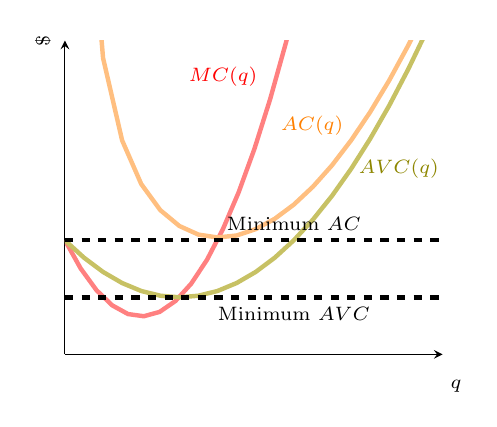
\begin{tikzpicture}\scriptsize  
	\begin{axis}[scale=0.7,
		xlabel=$q$,
		ylabel=$\$$,
		%grid=major,
		legend pos=outer north east,
		axis lines=center,
		enlarge x limits={rel=0.1, upper},
		enlarge y limits={rel=0.1, upper},
		every axis y label/.style={at={(axis description cs:-0.1,1)},rotate=90,anchor=north},
		every axis x label/.style={at={(axis description cs:1,-0.1)},anchor=west},
		ticks=none,
		ymax=20,
		ymin=0,
		xmin=0,
		]
		\addplot[ultra thick, domain=0:8,red!50, samples=30, name path=mc]{3*x^2-8*x+8};
		\addplot[ultra thick, domain=0:8,orange!50]{x^2-4*x+8+10/x};
		\addplot[ultra thick, domain=0:8,olive!50]{x^2-4*x+8};
		%\addplot[thick, domain=0:8,black]{10/x};
		%\addlegendentry{$AFC(q)=\frac{10}{y}$}
		\draw[ultra thick, dashed] (axis cs:0,8)--node[above]{Minimum $AC$}(axis cs:8,8);
		\draw[ultra thick, dashed] (axis cs:0,4)--node[below]{Minimum $AVC$}(axis cs:8,4);
		\draw[red] (axis cs:3.5,19.5)node[left]{$MC(q)$};
		\draw[orange] (axis cs:5,16)node[left]{$AC(q)$};
		\draw[olive] (axis cs:5,13)node[right]{$AVC(q)$};
	\end{axis}
	\end{tikzpicture}	
	\caption{The relationship between average and marginal}
	\end{figure}
	
	\clearpage 
	
 	\item In the long run, firms can change all factors of production (e.g. can choose $k$)
 	\begin{itemize}
 		\item Separate short run average cost curves for each hypothetical amount of $k$
 		\item In long run, firm chooses $k$ (and associated SRAC curve) to minimize cost at desired output level 
 		\item Long run average cost curve ``envelopes'' the lowest parts of all SRAC curves
 	\end{itemize}
 	\begin{figure}[h!]
 	\centering 
	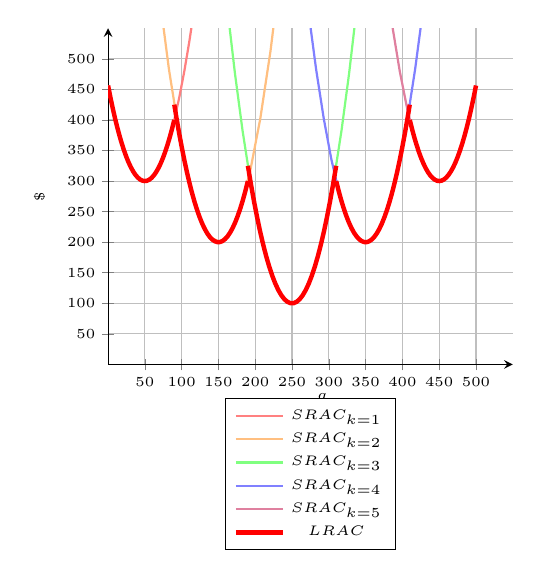
\begin{tikzpicture}\tiny  
	\begin{axis}[scale=0.75,
		xlabel=$q$,
		ylabel=$\$$,
		grid=major,
		legend style={at={(0.5,-0.1)},anchor=north},
		ymin=0,
		xtick={0,50,100,...,500},
		ytick={0,50,100,...,500},
				axis lines=middle, 
		enlarge x limits={rel=0.1, upper},
		enlarge y limits={rel=0.1, upper},
		every axis y label/.style={at={(axis description cs:-0.2,0.5)},rotate=90,anchor=north},
		every axis x label/.style={at={(axis description cs:0.5,-0.1)},anchor=west},
		ymax=500,
		xmax=500,
		xmin=0]
		\addplot[thick, domain=0:200,red!50, samples=30]{(0.25*x-12.5)^(2)+300};
		\addlegendentry{$SRAC_{k=1}$}
		%\addplot[thick, domain=0:300,red!50, samples=30]{(0.25*x-25)^(2)+250};
		\addplot[thick, domain=0:400,orange!50, samples=30]{(0.25*x-37.5)^(2)+200};
		\addlegendentry{$SRAC_{k=2}$}
		%\addplot[thick, domain=100:400,red!50, samples=30]{(0.25*x-50)^(2)+150};
		\addplot[thick, domain=100:400,green!50, samples=30]{(0.25*x-62.5)^(2)+100};
		\addlegendentry{$SRAC_{k=3}$}
		%\addplot[thick, domain=100:400,red!50, samples=30]{(0.25*x-75)^(2)+150};
		\addplot[thick, domain=200:500,blue!50, samples=30]{(0.25*x-87.5)^(2)+200};
		\addlegendentry{$SRAC_{k=4}$}
		%\addplot[thick, domain=200:500,red!50, samples=30]{(0.25*x-100)^(2)+250};
		\addplot[thick, domain=200:500,purple!50, samples=30]{(0.25*x-112.5)^(2)+300};
		\addlegendentry{$SRAC_{k=5}$}
		%LR
				\addplot[ultra thick, domain=0:90,red, samples=30]{(0.25*x-12.5)^(2)+300};
				\addlegendentry{$LRAC$}
		\addplot[ultra thick, domain=90:190,red, samples=30]{(0.25*x-37.5)^(2)+200};
		\addplot[ultra thick, domain=190:310,red, samples=30]{(0.25*x-62.5)^(2)+100};
		\addplot[ultra thick, domain=310:410,red, samples=30]{(0.25*x-87.5)^(2)+200};
		\addplot[ultra thick, domain=410:500,red, samples=30]{(0.25*x-112.5)^(2)+300};
	\end{axis}
	\end{tikzpicture}
	\caption{The relationship between short and long run average cost curves}
	\end{figure}
	\item \textbf{Economies of scale}: the economic relationship between how average cost scales with output 
	\begin{itemize}
		\item Economies of scale: average costs fall with output
		\item Diseconomies of scale: average costs rise with output 
		\item Constant economies of scale: costs do not vary with output
			\item Minimum efficient scale (MES): $q$ with lowest $AC(q)$
	\end{itemize} 
	\begin{figure}[h!]
		\centering 
				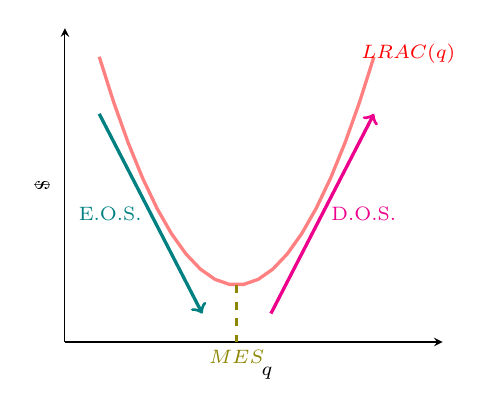
\begin{tikzpicture}\scriptsize 
	\begin{axis}[clip=false,
		scale=0.7,
		xlabel=$q$,
		ylabel=\$,
		grid=none,
		legend style={at={(0.5,-0.3)},anchor=north},
		ymin=0,
		ymax=20,
		xmax=10,
		xmin=0,
		ticks=none,
		axis lines=middle, 
		enlarge x limits={rel=0.1, upper},
		enlarge y limits={rel=0.1, upper},
		every axis y label/.style={at={(axis description cs:-0.1,0.5)},rotate=90,anchor=north},
		every axis x label/.style={at={(axis description cs:0.5,-0.1)},anchor=west},
		]
		\addplot[very thick, red!50, domain=1:9, samples=20]{(x-5)^(2)+4};
		\draw[red] (axis cs:10,19)node[above]{$LRAC(q)$};
		\draw[thick, dashed, olive] (axis cs:5,4)--(axis cs:5,0)node[below]{$MES$};
		\draw[very thick, teal, ->](axis cs:1,16)--node[left]{E.O.S.}(axis cs:4,2);
		\draw[very thick, magenta, ->](axis cs:6,2)--node[right]{D.O.S.}(axis cs:9,16);
	\end{axis}
		\end{tikzpicture}	
	\end{figure}
	\end{itemize} 
\end{itemize}

\clearpage 

\subsection*{Revenues}

\begin{itemize}
	\item \emph{Competitive} price-taking firm's demand is \emph{perfectly elastic} at the market-determined price
	\begin{table}[h!]
		\centering
		\begin{tabular}{cc}
		``Representative'' Firm & Industry\\
					\begin{tikzpicture}[scale=.35]\scriptsize
				\draw[->] (0,0) -- (11,0) coordinate (x axis) node[right]{$q$};
 				\draw[->] (0,0) -- (0,11) coordinate (y axis) node[above]{$p$};	
				\draw[very thick,blue!50] (0,5)node[left]{\textcolor{black}{$p^*$}} --(10,5) node[right] {$D^f$};
 			\end{tikzpicture}
		&
			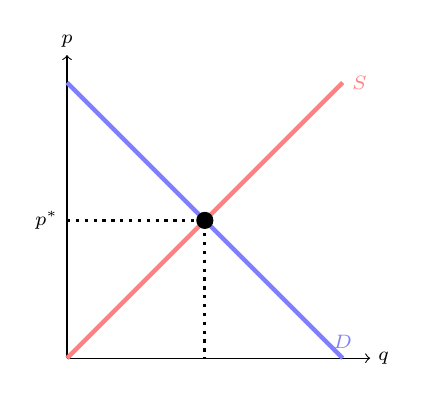
\begin{tikzpicture}[scale=.35]\scriptsize
				\draw[->] (0,0) -- (11,0) coordinate (x axis) node[right]{$q$};
 				\draw[->] (0,0) -- (0,11) coordinate (y axis) node[above]{$p$};	
				\draw[ultra thick,blue!50] (0,10) --(10,0) node[above] {$D$};
				\draw[ultra thick,red!50](0,0) -- (10,10)node[right]{$S$};	
				\draw[very thick, fill=black](5,5) circle (0.25cm);
				\draw[very thick, dotted](0,5)node[left]{$p^*$}--(5,5)--(5,0);
 			\end{tikzpicture}\\
		\end{tabular}
	\end{table}
	\item Total revenue 
	\begin{equation*}
	R(q)=pq	
	\end{equation*}
	\begin{itemize}
		\item Average Revenue: revenue per unit (aka price)
		\begin{equation*}
		AR(q)=p	
		\end{equation*}
		\item Marginal Revenue: how revenues change with one more output
		\begin{equation*}
		MR(q)=\frac{\Delta R(q)}{\Delta q}	
		\end{equation*}
		\begin{itemize}
			\item For a \emph{price-taking} firm in a \emph{competitive} market, Demand$=AR(q)=MR(q)=p$
		\end{itemize}
		
		\begin{table}[h!]
			\centering 
			\begin{tabular}{cc}
							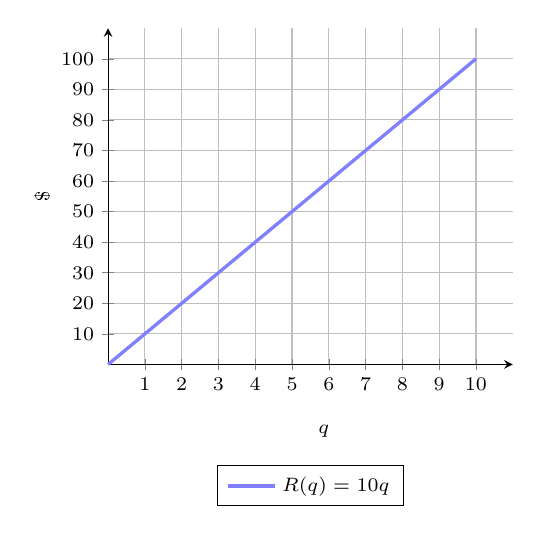
\begin{tikzpicture}\scriptsize 
	\begin{axis}[clip=false,
		scale=0.75,
		xlabel=$q$,
		ylabel=\$,
		grid=major,
		legend style={at={(0.5,-0.3)},anchor=north},
		ymin=0,
		ymax=100,
		xmax=10,
		xmin=0,
		xtick={0,1,...,10},
		ytick={0,10,...,100},
		axis lines=middle, 
		enlarge x limits={rel=0.1, upper},
		enlarge y limits={rel=0.1, upper},
		every axis y label/.style={at={(axis description cs:-0.2,0.5)},rotate=90,anchor=north},
		every axis x label/.style={at={(axis description cs:0.5,-0.2)},anchor=west},
		]
		\addplot[very thick, blue!50, domain=0:10, samples=20]{10*x};
		\addlegendentry{$R(q)=10q$}
		\end{axis} 
 			\end{tikzpicture}
&
						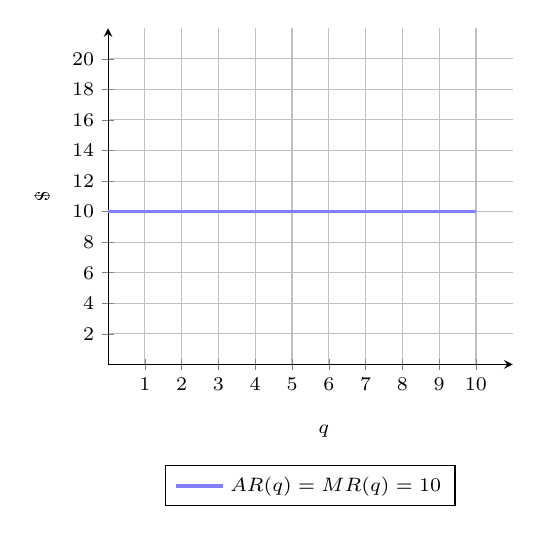
\begin{tikzpicture}\scriptsize 
	\begin{axis}[clip=false,
		scale=0.75,
		xlabel=$q$,
		ylabel=\$,
		grid=major,
		legend style={at={(0.5,-0.3)},anchor=north},
		ymin=0,
		ymax=20,
		xmax=10,
		xmin=0,
		xtick={0,1,...,10},
		ytick={0,2,...,20},
		axis lines=middle, 
		enlarge x limits={rel=0.1, upper},
		enlarge y limits={rel=0.1, upper},
		every axis y label/.style={at={(axis description cs:-0.2,0.5)},rotate=90,anchor=north},
		every axis x label/.style={at={(axis description cs:0.5,-0.2)},anchor=west},
		]
		\addplot[very thick, blue!50, domain=0:10, samples=20]{10};
		\addlegendentry{$AR(q)=MR(q)=10$}
		\end{axis} 
 			\end{tikzpicture}\\
			\end{tabular}
			\caption{Firm's total (left) and per-unit (right) revenues}
		\end{table}
	\end{itemize} 
	\end{itemize} 
\end{itemize}

\clearpage 

\subsection*{Profits}

\begin{itemize}
	\item A \textbf{competitive market}: 
		\begin{itemize}
			\item Firms' products are perfect substitutes 
		\item Firms are price-takers, none can affect the market price
		\item Market entry and exit is costless 
		\end{itemize}
	\item Firm chooses profit maximizing quantity $q^*$: 
	\begin{equation*}
	\pi_{max} \text{ at $q^*$ where }MR(q)=MC(q)	
	\end{equation*}
	\begin{table}[h!]
	\begin{tabular}{cc}
				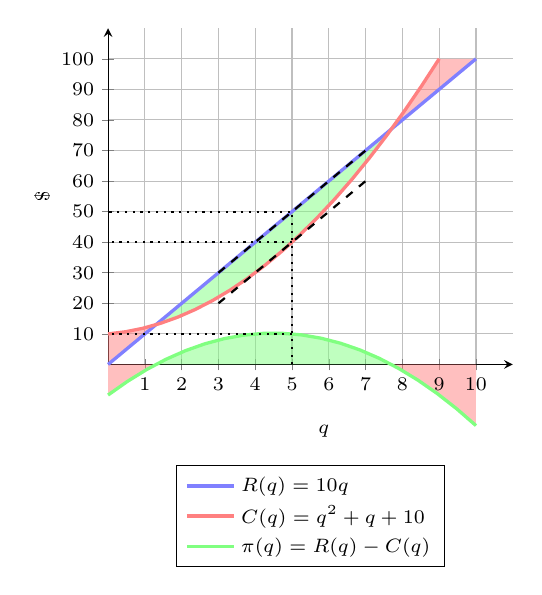
\begin{tikzpicture}\scriptsize 
	\begin{axis}[clip=false,
		scale=0.75,
		xlabel=$q$,
		ylabel=\$,
		grid=major,
		legend style={at={(0.5,-0.3)},anchor=north},
		legend cell align=left,
		ymin=0,
		ymax=100,
		xmax=10,
		xmin=0,
		xtick={0,1,...,10},
		ytick={0,10,...,100},
		axis lines=middle, 
		enlarge x limits={rel=0.1, upper},
		enlarge y limits={rel=0.1, upper},
		every axis y label/.style={at={(axis description cs:-0.2,0.5)},rotate=90,anchor=north},
		every axis x label/.style={at={(axis description cs:0.5,-0.2)},anchor=west},
		]
		\addplot[name path=r, very thick, blue!50, domain=0:10, samples=20]{10*x};
		\addlegendentry{$R(q)=10q$}
		\addplot[name path=c, very thick, red!50, domain=0:9, samples=20]{x^2+x+10};
		\addlegendentry{$C(q)=q^2+q+10$}
		\addplot[name path=p, very thick, green!50, domain=0:10, samples=20]{9*x-x^2-10};
		\addlegendentry{$\pi(q)=R(q)-C(q)$}
		\path[name path=axis] (axis cs:0,0) -- (axis cs:10,0);
    \addplot fill between[of=r and c, split,
    every even segment/.style = {red!50, opacity=0.5},
    every odd segment/.style  = {green!50, opacity=0.5}];	
    \addplot fill between[of=p and axis, split, 
    every even segment/.style = {red!50, opacity=0.5},
    every odd segment/.style  = {green!50, opacity=0.5}];	
    	\draw[thick, dashed] (axis cs:3,20)--(axis cs:7,60);
    	\draw[thick, dashed] (axis cs:3,30)--(axis cs:7,70);
		\draw[thick, dotted] (axis cs:5,0)--(axis cs:5,50)--(axis cs:0,50);
		\draw[thick, dotted] (axis cs:5,40)--(axis cs:0,40);
		\draw[thick, dotted] (axis cs:5,10)--(axis cs:0,10);
		\end{axis} 
 			\end{tikzpicture}
	&
				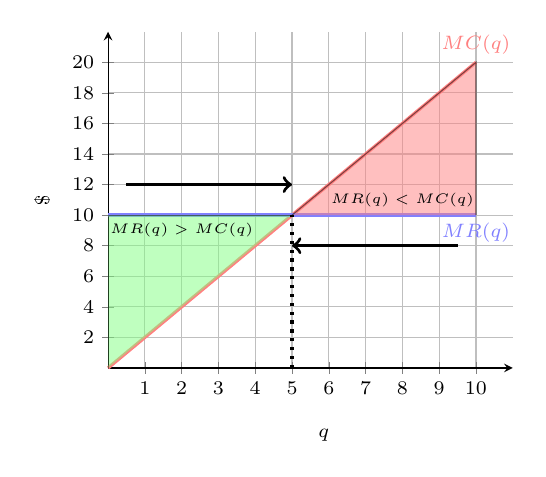
\begin{tikzpicture}\scriptsize 
	\begin{axis}[clip=false,
		scale=0.75,
		xlabel=$q$,
		ylabel=\$,
		grid=major,
		legend style={at={(0.5,-0.3)},anchor=north},
		legend cell align=left,
		ymin=0,
		ymax=20,
		xmax=10,
		xmin=0,
		xtick={0,1,...,10},
		ytick={0,2,...,20},
		axis lines=middle, 
		enlarge x limits={rel=0.1, upper},
		enlarge y limits={rel=0.1, upper},
		every axis y label/.style={at={(axis description cs:-0.2,0.5)},rotate=90,anchor=north},
		every axis x label/.style={at={(axis description cs:0.5,-0.2)},anchor=west},
		]
		\addplot[very thick, red!50, domain=0:10, samples=20]{2*x};
		\draw[red!50] (axis cs: 10,20)node[above]{$MC(q)$};
		\addplot[very thick, blue!50, domain=0:10, samples=20]{10};
		\draw[blue!50] (axis cs: 10,10)node[below]{$MR(q)$};
		\draw[fill=green!50,opacity=0.5](axis cs:0,0)--(axis cs:0,10)--(axis cs:5,10);
		\draw (axis cs:2,10)node[below]{\tiny $MR(q)>MC(q)$};
		\draw[fill=red!50, opacity=0.5](axis cs:5,10)--(axis cs:10,20)--(axis cs:10,10);
		\draw (axis cs:8,10)node[above]{\tiny $MR(q)<MC(q)$};
		\draw[very thick, black, ->] (axis cs:0.5,12)--(axis cs: 5,12);
		\draw[very thick, black, ->] (axis cs:9.5,8)--(axis cs:5,8);
		\draw[very thick, dotted] (axis cs:5,0)--(axis cs:5,10);
		\end{axis} 
 			\end{tikzpicture}\\
	\end{tabular}
	\caption{Finding maximum profits (totals on left, per unit on right)} 
	\end{table}
	
\clearpage 

	\item Profit is revenues minus costs: 
	\begin{align*}
	\pi &= R(q) - C(q)\\
	\pi & =q[p-AC(q)]\\ 	
	\end{align*}

	\begin{figure}[h!]
		\centering 
			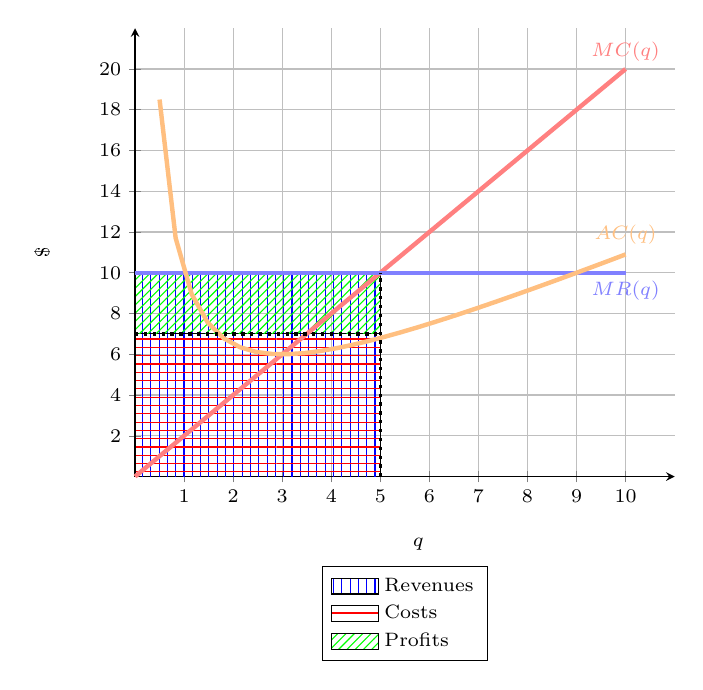
\begin{tikzpicture}\scriptsize 
	\begin{axis}[clip=false,
		scale=1,
		xlabel=$q$,
		ylabel=\$,
		grid=major,
		legend style={at={(0.5,-0.2)},anchor=north},
		legend cell align=left,
		ymin=0,
		ymax=20,
		xmax=10,
		xmin=0,
		xtick={0,1,...,10},
		ytick={0,2,...,20},
		axis lines=middle, 
		enlarge x limits={rel=0.1, upper},
		enlarge y limits={rel=0.1, upper},
		every axis y label/.style={at={(axis description cs:-0.2,0.5)},rotate=90,anchor=north},
		every axis x label/.style={at={(axis description cs:0.5,-0.15)},anchor=west},
		]
		%\draw[blue, pattern=north east lines, pattern color=blue] (0,0) -- (0,10) -- (5,10)--(5,0); 
		\addplot[pattern=vertical lines, area legend, pattern color=blue] coordinates {(0,0) (0,10) (5,10) (5,0)};
		\addlegendentry{Revenues}
		\addplot[pattern=horizontal lines, area legend, pattern color=red] coordinates {(0,0) (0,7) (5,7) (5,0)};
		\addlegendentry{Costs}
		\addplot[pattern=north east lines,area legend, pattern color=green] coordinates {(0,7) (0,10) (5,10) (5,7)};
		\addlegendentry{Profits}
		\addplot[ultra thick, red!50, domain=0:10, samples=20]{2*x};
		\draw[red!50] (axis cs: 10,20)node[above]{$MC(q)$};
		\addplot[ultra thick, blue!50, domain=0:10, samples=20]{10};
		\draw[blue!50] (axis cs: 10,10)node[below]{$MR(q)$};
		\addplot[ultra thick, domain=0.5:10,orange!50, samples=30]{x+9/x};
		\draw[orange!50] (axis cs: 10,11)node[above]{$AC(q)$};
		\draw[very thick, dotted] (axis cs:5,0)--(axis cs:5,10);
		\draw[very thick, dotted] (axis cs:0,7)--(axis cs:5,7);
 		\end{axis} 
 			\end{tikzpicture}
	\end{figure}
	\item Firm breaks even where $p=AC(q)$
	\begin{itemize}
		\item Firm's break even price is the minimum of $AC(q)$ curve (where $AC(q)=MC(q)$)	
	\end{itemize}
	\item Firm earns losses where $p<AC(q)$
	\begin{itemize}
		\item \textbf{Short run}: firm stays in market
		\begin{itemize}
			\item Firm continues to produce (at a loss) if 
			\begin{equation*}
			p \geq AVC	
			\end{equation*}
			\item Firm \textbf{shuts down} and produces $q^*=0$ if
			\begin{equation*}
			p < AVC	
			\end{equation*}
			\item Firm's shut down price is the minimum of $AVC(q)$ curve (where $AVC(q)=MC(q)$) 
		\end{itemize}
		\item \textbf{Long run}: firm exits market 
	\end{itemize} 

\clearpage 

	\item Firm's Supply:
	\begin{table}[h!] 
		\centering 
		\begin{tabular}{cc}
				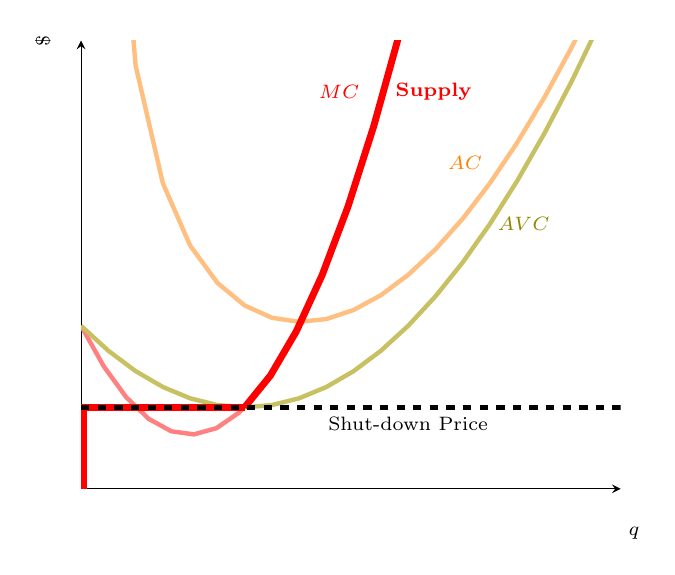
\begin{tikzpicture}\scriptsize  
	\begin{axis}[
		xlabel=$q$,
		ylabel=$\$$,
		%grid=major,
		legend pos=outer north east,
		axis lines=center,
		enlarge x limits={rel=0.1, upper},
		enlarge y limits={rel=0.1, upper},
		every axis y label/.style={at={(axis description cs:-0.1,1)},rotate=90,anchor=north},
		every axis x label/.style={at={(axis description cs:1,-0.1)},anchor=west},
		ticks=none,
		ymax=20,
		ymin=0,
		xmin=0,
		]
		\addplot[ultra thick, domain=0:8,red!50, samples=30]{3*x^2-8*x+8};
		\addplot[ultra thick, domain=0:8,orange!50]{x^2-4*x+8+10/x};
		\addplot[ultra thick, domain=0:8,olive!50]{x^2-4*x+8};
		%\addplot[thick, domain=0:8,black]{10/x};
		%\addlegendentry{$AFC(q)=\frac{10}{y}$}
		\addplot[line width=2.5, domain=2:8,red, samples=20]{3*x^2-8*x+8};
		%\draw[ultra thick, red] (axis cs:0,0)--(axis cs:0,4);
		\draw[line width=2.5, red] (axis cs:0.03,0)--(axis cs:0.03,4);
		\draw[line width=2.5, red] (axis cs:0,4)--(axis cs:2,4);
				\draw[red] (axis cs:3.5,19.5)node[left]{$MC$};
		\draw[red] (axis cs:3.75,19.5)node[right]{\textbf{Supply}};
		\draw[orange] (axis cs:5,16)node[left]{$AC$};
		\draw[olive] (axis cs:5,13)node[right]{$AVC$};
		\draw[ultra thick, dashed] (axis cs:0,4)--node[below]{Shut-down Price}(axis cs:8,4);
	\end{axis}
	\end{tikzpicture}
	&
				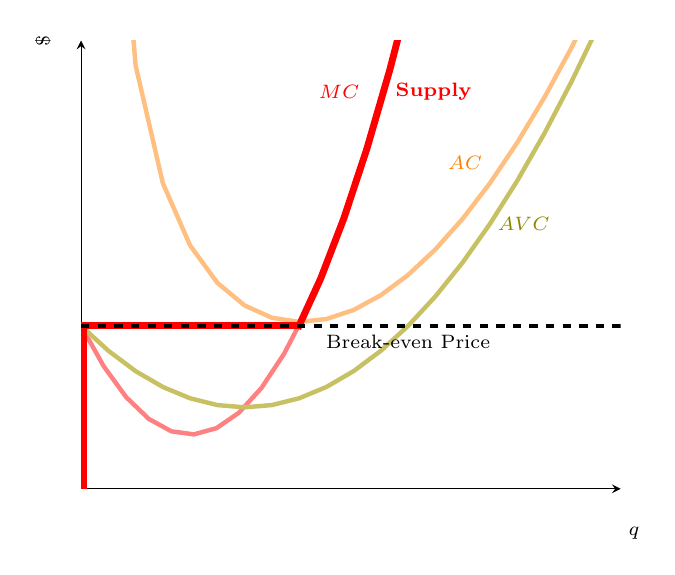
\begin{tikzpicture}\scriptsize  
	\begin{axis}[
		xlabel=$q$,
		ylabel=$\$$,
		%grid=major,
		legend pos=outer north east,
		axis lines=center,
		enlarge x limits={rel=0.1, upper},
		enlarge y limits={rel=0.1, upper},
		every axis y label/.style={at={(axis description cs:-0.1,1)},rotate=90,anchor=north},
		every axis x label/.style={at={(axis description cs:1,-0.1)},anchor=west},
		ticks=none,
		ymax=20,
		ymin=0,
		xmin=0,
		]
		\addplot[ultra thick, domain=0:8,red!50, samples=30]{3*x^2-8*x+8};
		\addplot[ultra thick, domain=0:8,orange!50]{x^2-4*x+8+10/x};
		\addplot[ultra thick, domain=0:8,olive!50]{x^2-4*x+8};
		%\addplot[thick, domain=0:8,black]{10/x};
		%\addlegendentry{$AFC(q)=\frac{10}{y}$}
		\addplot[line width=2.5, domain=2.65:8,red, samples=20]{3*x^2-8*x+8};
		%\draw[ultra thick, red] (axis cs:0,0)--(axis cs:0,4);
		\draw[line width=2.5, red] (axis cs:0.03,0)--(axis cs:0.03,8);
		\draw[line width=2.5, red] (axis cs:0,8)--(axis cs:2.65,8);
				\draw[red] (axis cs:3.5,19.5)node[left]{$MC$};
		\draw[red] (axis cs:3.75,19.5)node[right]{\textbf{Supply}};
		\draw[orange] (axis cs:5,16)node[left]{$AC$};
		\draw[olive] (axis cs:5,13)node[right]{$AVC$};
		\draw[ultra thick, dashed] (axis cs:0,8)--node[below]{Break-even Price}(axis cs:8,8);
	\end{axis}
	\end{tikzpicture}
	\\
	\end{tabular}
	\caption{Firm's Supply in Short Run (left) and Long Run (right)}
	\end{table}
			\begin{align*}
	\text{Firm's Short Run Inverse Supply}&= \left\{
 		 \begin{array}{ll}
    		p=MC(q) & \text{if } p \geq AVC \\
   			q=0 & \text{If } p < AVC\\
  		\end{array}
  		\right.	\\
	\text{Firm's Long Run Inverse Supply}&= \left\{
 		 \begin{array}{ll}
    		p=MC(q) & \text{if } p \geq AC \\
   			q=0 & \text{If } p < AC\\
  		\end{array}
  		\right.	\\
	\end{align*}
	\item Industry equilibrium: 
	\begin{itemize}
		\item If firms earn $\pi>0$ in short run: firms enter over long run
		\item If firms earn $\pi<0$ in short run: firms exit over long run
		\item \textbf{Long run equilibrium: $\pi=0$ at $p=AC(q)=MC(q)$ for all firms!}
	\end{itemize}
	\item Industry supply curve is sum of all firms' marginal cost curves above $AVC_{min}$
	\begin{table}[h!]
		\centering 
		\begin{tabular}{ccc}
		Firm 1 & Firm 2 & Industry\\
						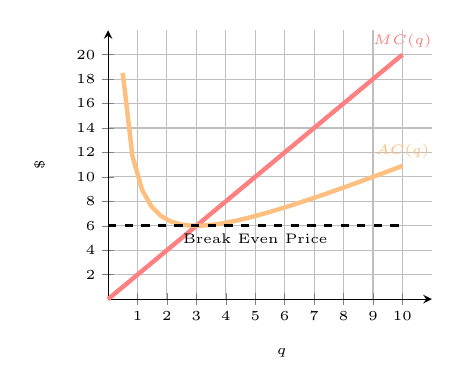
\begin{tikzpicture}\tiny 
	\begin{axis}[scale=0.6,
	clip=false,
		xlabel=$q$,
		ylabel=$\$$,
		%grid=major,
		legend pos=outer north east,
		axis lines=center,
		grid=major,
				enlarge x limits={rel=0.1, upper},
		enlarge y limits={rel=0.1, upper},
		every axis y label/.style={at={(axis description cs:-0.1,1)},rotate=90,anchor=north},
		every axis x label/.style={at={(axis description cs:1,-0.1)},anchor=west},
		ymin=0,
		ymax=20,
		xmax=10,
		xmin=0,
		xtick={0,1,...,10},
		ytick={0,2,...,20},
		axis lines=middle, 
		enlarge x limits={rel=0.1, upper},   
		enlarge y limits={rel=0.1, upper},
		every axis y label/.style={at={(axis description cs:-0.25,0.5)},rotate=90,anchor=north},
		every axis x label/.style={at={(axis description cs:0.5,-0.2)},anchor=west},
		]
		%\draw<2->[blue, pattern=north east lines, pattern color=blue] (0,0) -- (0,10) -- (5,10)--(5,0); 
		\addplot[ultra thick, red!50, domain=0:10, samples=20]{2*x};
		\draw[red!50] (axis cs: 10,20)node[above]{$MC(q)$};
		\addplot[ultra thick, domain=0.5:10,orange!50, samples=30]{x+9/x};
		\draw[orange!50] (axis cs: 10,11)node[above]{$AC(q)$};
		%\addplot[ultra thick, domain=0:10,olive!50]{x};
		%\draw[olive!50] (axis cs: 10,9)node[below]{$AVC(q)$};
		\draw[very thick, dashed, black] (axis cs:0,6)--node[below]{Break Even Price}(axis cs:10,6);
		\end{axis} 
 			\end{tikzpicture}
 			&
 						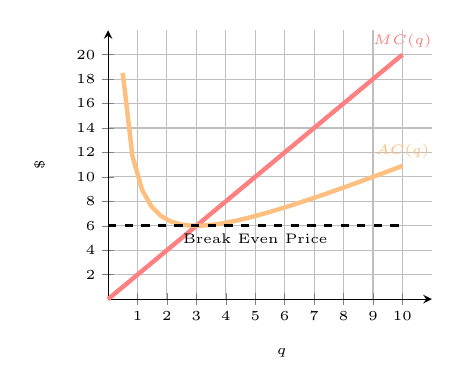
\begin{tikzpicture}\tiny 
	\begin{axis}[scale=0.6,
	clip=false,
		xlabel=$q$,
		ylabel=$\$$,
		%grid=major,
		legend pos=outer north east,
		axis lines=center,
		grid=major,
				enlarge x limits={rel=0.1, upper},
		enlarge y limits={rel=0.1, upper},
		every axis y label/.style={at={(axis description cs:-0.1,1)},rotate=90,anchor=north},
		every axis x label/.style={at={(axis description cs:1,-0.1)},anchor=west},
		ymin=0,
		ymax=20,
		xmax=10,
		xmin=0,
		xtick={0,1,...,10},
		ytick={0,2,...,20},
		axis lines=middle, 
		enlarge x limits={rel=0.1, upper},   
		enlarge y limits={rel=0.1, upper},
		every axis y label/.style={at={(axis description cs:-0.25,0.5)},rotate=90,anchor=north},
		every axis x label/.style={at={(axis description cs:0.5,-0.2)},anchor=west},
		]
		%\draw<2->[blue, pattern=north east lines, pattern color=blue] (0,0) -- (0,10) -- (5,10)--(5,0); 
		\addplot[ultra thick, red!50, domain=0:10, samples=20]{2*x};
		\draw[red!50] (axis cs: 10,20)node[above]{$MC(q)$};
		\addplot[ultra thick, domain=0.5:10,orange!50, samples=30]{x+9/x};
		\draw[orange!50] (axis cs: 10,11)node[above]{$AC(q)$};
		%\addplot[ultra thick, domain=0:10,olive!50]{x};
		%\draw[olive!50] (axis cs: 10,9)node[below]{$AVC(q)$};
		\draw[very thick, dashed, black] (axis cs:0,6)--node[below]{Break Even Price}(axis cs:10,6);
		\end{axis} 
 			\end{tikzpicture}
	&
 						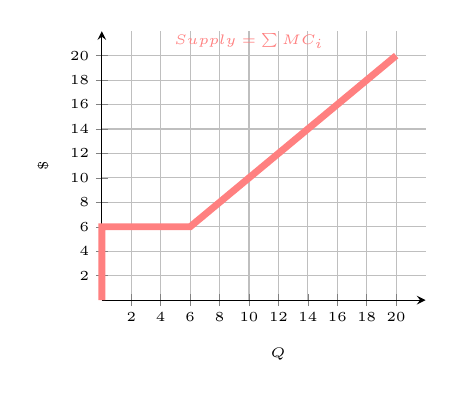
\begin{tikzpicture}\tiny 
	\begin{axis}[scale=0.6,
		clip=false,
		xlabel=$Q$,
		ylabel=$\$$,
		%grid=major,
		legend pos=outer north east,
		axis lines=center,
		grid=major,
				enlarge x limits={rel=0.1, upper},
		enlarge y limits={rel=0.1, upper},
		every axis y label/.style={at={(axis description cs:-0.2,1)},rotate=90,anchor=north},
		every axis x label/.style={at={(axis description cs:1,-0.1)},anchor=west},
		ymin=0,
		ymax=20,
		xmax=20,
		xmin=0,
		xtick={0,2,...,20},
		ytick={0,2,...,20},
		axis lines=middle, 
		enlarge x limits={rel=0.1, upper},   
		enlarge y limits={rel=0.1, upper},
		every axis y label/.style={at={(axis description cs:-0.22,0.5)},rotate=90,anchor=north},
		every axis x label/.style={at={(axis description cs:0.5,-0.2)},anchor=west},
		]
		%\draw<2->[blue, pattern=north east lines, pattern color=blue] (0,0) -- (0,10) -- (5,10)--(5,0); 
		\draw[line width=2.5, red!50](axis cs:0,0)--(axis cs:0,6)--(axis cs:6,6)--(axis cs:20,20);
		\addplot[opacity=0]{x};
		\draw[red!50] (axis cs: 10,20)node[above]{$Supply=\sum MC_i$};
		\end{axis} 
 			\end{tikzpicture}\\
		\end{tabular}
	\end{table}
	\item Firms may have different cost structures due to \textbf{economic rents} -- returns above opportunity cost needed to bring firm online 
	\begin{itemize}
		\item A scarce factor of production (e.g. talent, location, intellectual property, political favors, etc)
		\item Lowers costs for firm relative to other firms 
		\item Other firms willing to bid up price of scarce rent-generating factor (to earn advantage)
		\item Prices of rent-generating factors get bid up until firm profits fall to zero! 
		\item Owner of scarce factor earns higher income due to economic rents
	\end{itemize}

\clearpage 

	\item Entry effects \& External Economies 
	\begin{itemize}
		\item \textbf{Constant cost industry (no external economies)}: increase in output/entry in industry has no effect on costs for all firms in industry
	\begin{table}[h!]
		\centering 
		\begin{tabular}{cc}
			``Representative'' Firm & Industry\\
			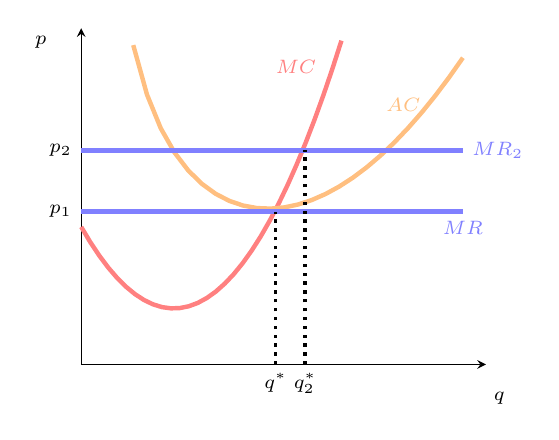
\begin{tikzpicture}\scriptsize 
			\begin{axis}[clip=false,
	scale=0.75,
		xlabel=$q$,
		ylabel=$p$,
		%grid=major,
		legend pos=outer north east,
		axis lines=center,
				enlarge x limits={rel=0.1, upper},
		enlarge y limits={rel=0.1, upper},
		every axis y label/.style={at={(axis description cs:-0.1,1)},anchor=north},
		every axis x label/.style={at={(axis description cs:1,-0.1)},anchor=west},
		ticks=none,
		ymax=20,
		ymin=0,
		]
		\addplot[ultra thick, domain=0:3.75,red!50, samples=30, name path=mc]{3*x^2-8*x+9};
		\addplot[ultra thick, domain=0.75:5.5,orange!50]{x^2-4*x+10+10/x};
		%\addplot[ultra thick, domain=0:8,olive!50]{x^2-4*x+9};
		%\addplot[thick, domain=0:8,black]{10/x};
		%\addlegendentry{$AFC(q)=\frac{10}{y}$}
		\draw[ultra thick, blue!50, name path=mr] (axis cs: 0,10)node[left]{\textcolor{black}{$p_1$}}--(axis cs:5.5,10)node[below]{$MR$};
		%\addplot[thick, domain=0:8,black]{10/x};
		%\addlegendentry{$AFC(q)=\frac{10}{y}$}
		%\draw[ultra thick, red] (axis cs:0,0)--(axis cs:0,4);
		\draw[very thick, dotted](axis cs:2.8,0)node[below]{$q^*$}--(axis cs:2.8,10);
		\draw[red!50] (axis cs:3.5,19.5)node[left]{$MC$};
		\draw[orange!50] (axis cs:5,17)node[left]{$AC$};
		%\draw[olive] (axis cs:5,13)node[right]{$AVC$};
		\draw[ultra thick, blue!50] (axis cs: 0,14)node[left]{\textcolor{black}{$p_2$}}--(axis cs:5.5,14)node[right]{$MR_2$};
		\draw[very thick, dotted](axis cs:3.225,0)node[below]{$q_2^*$}--(axis cs:3.225,14);
		%\draw[green, fill=green, opacity=0.5] (axis cs:0,10.75)--(axis cs:0,14)--(axis cs:3.225,14)--(axis cs:3.225,10.75);
		\end{axis}
 			\end{tikzpicture}
&
			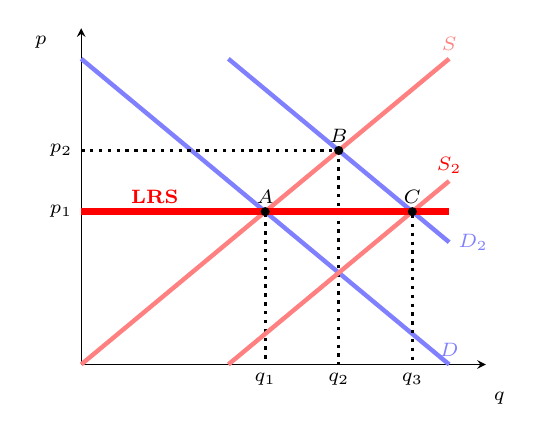
\begin{tikzpicture}\scriptsize  
				\begin{axis}[clip=false,
	scale=0.75,
		xlabel=$q$,
		ylabel=$p$,
		%grid=major,
		legend pos=outer north east,
		axis lines=center,
				enlarge x limits={rel=0.1, upper},
		enlarge y limits={rel=0.1, upper},
		every axis y label/.style={at={(axis description cs:-0.1,1)},anchor=north},
		every axis x label/.style={at={(axis description cs:1,-0.1)},anchor=west},
		ticks=none,
		ymax=10,
		ymin=0,
		]
		\addplot[ultra thick, domain=0:10,red!50, samples=30]{x};
		\addplot[ultra thick, domain=0:10,blue!50]{10-x};
		\draw[ultra thick, blue!50] (axis cs:4,10)--(axis cs:10,4)node[right]{$D_2$};
		\draw[very thick, dotted] (axis cs:0,5)node[left]{$p_1$}--(axis cs:5,5)--(axis cs:5,0)node[below]{$q_1$};
		\draw[blue!50] (axis cs:10,0)node[above]{$D$};
		\draw[red!50] (axis cs:10,10)node[above]{$S$};
		\draw[very thick, dotted] (axis cs:0,7)node[left]{$p_2$}--(axis cs:7,7)--(axis cs:7,0)node[below]{$q_2$};
		\draw[ultra thick, red!50] (axis cs:4,0)--(axis cs:10,6);
		\draw[red] (axis cs:10,6)node[above]{$S_2$};
		\draw[very thick, dotted] (axis cs:5,5)--(axis cs:9,5)--(axis cs:9,0)node[below]{$q_3$};
		\draw[line width=2.5, red] (axis cs:0,5)--(axis cs:10,5);
		\draw[red] (axis cs:2,5)node[above]{\textbf{LRS}};
		\draw[fill=black] (axis cs:5,5)circle(0.05cm)node[above]{$A$};
		\draw[fill=black] (axis cs:7,7)circle(0.05cm)node[above]{$B$};
		\draw[fill=black] (axis cs:9,5)circle(0.05cm)node[above]{$C$};
		\end{axis} 
 			\end{tikzpicture}\\
		\end{tabular}
	\end{table}
		\begin{itemize}
			\item \textbf{Short run}: $A \rightarrow B$: increase in demand, firms earn profit
			\item \textbf{Long run}: $B \rightarrow C$: profits attract entry
			\begin{itemize}
				\item Entry does not change costs
				\item Entry continues until price returns to $p_1$, where $p=AC(q)=MC(q)$ and $\pi=0$ for all firms
				\item Long run supply curve is perfectly elastic (horizontal)
			\end{itemize} 
		\end{itemize}
		\item \textbf{Increasing cost industry (external diseconomies)}: increase in output/entry in industry raises costs for all firms in industry
			\begin{table}[h!]
				\centering 
		\begin{tabular}{cc}
			``Representative'' Firm & Industry\\
			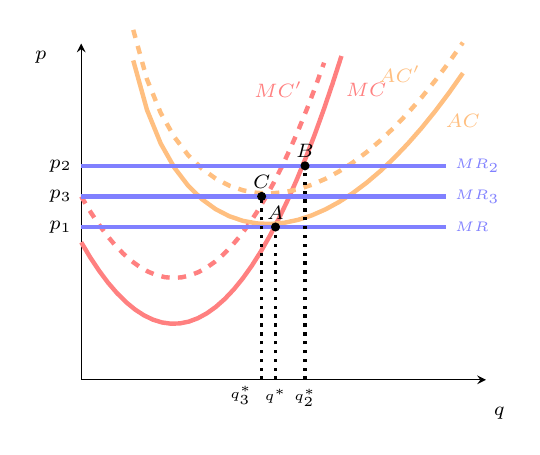
\begin{tikzpicture}\scriptsize 
			\begin{axis}[clip=false,
	scale=0.75,
		xlabel=$q$,
		ylabel=$p$,
		%grid=major,
		legend pos=outer north east,
		axis lines=center,
				enlarge x limits={rel=0.1, upper},
		enlarge y limits={rel=0.1, upper},
		every axis y label/.style={at={(axis description cs:-0.1,1)},anchor=north},
		every axis x label/.style={at={(axis description cs:1,-0.1)},anchor=west},
		ticks=none,
		ymax=20,
		ymin=0,
		]
		\addplot[ultra thick, domain=0:3.75,red!50, samples=30]{3*x^2-8*x+9};
		\addplot[ultra thick, domain=0.75:5.5,orange!50]{x^2-4*x+10+10/x};
		\addplot[ultra thick, dashed, domain=0:3.5,red!50, samples=30]{3*x^2-8*x+12};
		\addplot[ultra thick, dashed, domain=0.75:5.5,orange!50]{x^2-4*x+12+10/x};
		%\addplot[ultra thick, domain=0:8,olive!50]{x^2-4*x+9};
		%\addplot[thick, domain=0:8,black]{10/x};
		%\addlegendentry{$AFC(q)=\frac{10}{y}$}
		\draw[ultra thick, blue!50] (axis cs: 0,10)node[left]{\textcolor{black}{$p_1$}}--(axis cs:5.25,10)node[right]{\tiny $MR$};
		%\addplot[thick, domain=0:8,black]{10/x};
		%\addlegendentry{$AFC(q)=\frac{10}{y}$}
		%\draw[ultra thick, red] (axis cs:0,0)--(axis cs:0,4);
		\draw[very thick, dotted](axis cs:2.8,0)node[below]{\tiny $q^*$}--(axis cs:2.8,10);
		\draw[red!50] (axis cs:3.7,19)node[right]{$MC$};
		\draw[red!50] (axis cs:3.3,19)node[left]{$MC'$};
		\draw[orange!50] (axis cs:5.5,16)node[above]{$AC$};
		%\draw[olive] (axis cs:5,13)node[right]{$AVC$};
		\draw[ultra thick, blue!50] (axis cs: 0,14)node[left]{\textcolor{black}{$p_2$}}--(axis cs:5.25,14)node[right]{\tiny $MR_2$};
		\draw[very thick, dotted](axis cs:3.225,0)node[below]{\tiny $q_2^*$}--(axis cs:3.225,14);
		\draw[ultra thick, blue!50] (axis cs: 0,12)node[left]{\textcolor{black}{$p_3$}}--(axis cs:5.25,12)node[right]{\tiny $MR_3$};
		\draw[very thick, dotted](axis cs:2.6,0)node[below=0.2cm,left=0.0125cm]{\tiny $q_3^*$}--(axis cs:2.6,12);
		\draw[orange!50] (axis cs:5,20)node[left]{$AC'$};
		\draw[fill=black] (axis cs:2.8,10)circle(0.05cm)node[above]{$A$};
		\draw[fill=black] (axis cs:3.225,14)circle(0.05cm)node[above]{$B$};
		\draw[fill=black] (axis cs:2.6,12)circle(0.05cm)node[above]{$C$};
		\end{axis}
 			\end{tikzpicture}
&
			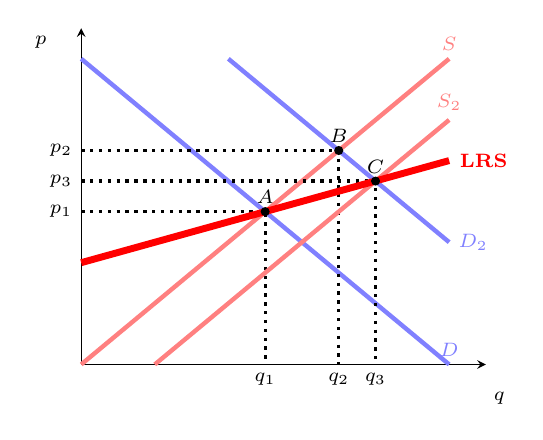
\begin{tikzpicture}\scriptsize  
				\begin{axis}[clip=false,
	scale=0.75,
		xlabel=$q$,
		ylabel=$p$,
		%grid=major,
		legend pos=outer north east,
		axis lines=center,
				enlarge x limits={rel=0.1, upper},
		enlarge y limits={rel=0.1, upper},
		every axis y label/.style={at={(axis description cs:-0.1,1)},anchor=north},
		every axis x label/.style={at={(axis description cs:1,-0.1)},anchor=west},
		ticks=none,
		ymax=10,
		ymin=0,
		]
		\addplot[ultra thick, domain=0:10,red!50, samples=30]{x};
		\addplot[ultra thick, domain=0:10,blue!50]{10-x};
		\draw[ultra thick, blue!50] (axis cs:4,10)--(axis cs:10,4)node[right]{$D_2$};
		\draw[very thick, dotted] (axis cs:0,5)node[left]{$p_1$}--(axis cs:5,5)--(axis cs:5,0)node[below]{$q_1$};
		\draw[blue!50] (axis cs:10,0)node[above]{$D$};
		\draw[red!50] (axis cs:10,10)node[above]{$S$};
		\draw[very thick, dotted] (axis cs:0,7)node[left]{$p_2$}--(axis cs:7,7)--(axis cs:7,0)node[below]{$q_2$};
		\draw[ultra thick, red!50] (axis cs:2,0)--(axis cs:10,8)node[above]{$S_2$};
		\draw[very thick, dotted] (axis cs:0,6)node[left]{$p_3$}--(axis cs:8,6)--(axis cs:8,0)node[below]{$q_3$};
		\draw[line width=2.5, red] (axis cs:0,3.33)--(axis cs:10,6.67)node[right]{\textbf{LRS}};
		\draw[fill=black] (axis cs:5,5)circle(0.05cm)node[above]{$A$};
		\draw[fill=black] (axis cs:7,7)circle(0.05cm)node[above]{$B$};
		\draw[fill=black] (axis cs:8,6)circle(0.05cm)node[above]{$C$};
		\end{axis} 
 			\end{tikzpicture}\\
		\end{tabular}
	\end{table}
		\begin{itemize}
			\item \textbf{Short run}: $A \rightarrow B$: increase in demand, firms earn profit
			\item \textbf{Long run}: $B \rightarrow C$: profits attract entry
			\begin{itemize}
				\item Entry raises costs to all firms (dashed curves) 
				\item Entry continues until price falls to $p_3$ (higher than $p_1$), where $p=AC(q)=MC(q)$ and $\pi=0$ for all firms
				\item Long run supply curve is upward sloping due to increased costs
			\end{itemize} 
		\end{itemize}
		
	\clearpage 
	
		\item \textbf{Decreasing cost industry (external economies)}: increase in output/entry in industry lowers costs for all firms in industry
	\begin{table}
		\centering 
		\begin{tabular}{cc}
			``Representative'' Firm & Industry\\
			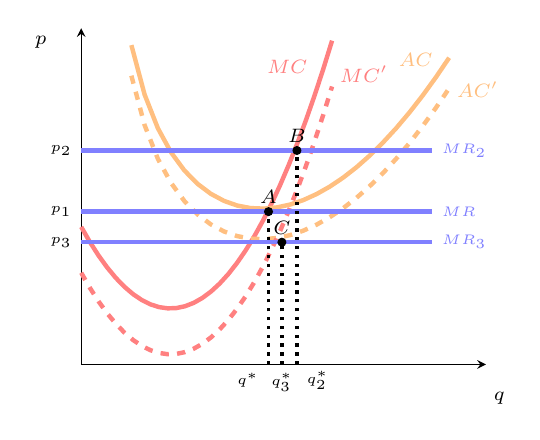
\begin{tikzpicture}\scriptsize  
			\begin{axis}[clip=false,
	scale=0.75,
		xlabel=$q$,
		ylabel=$p$,
		%grid=major,
		legend pos=outer north east,
		axis lines=center,
				enlarge x limits={rel=0.1, upper},
		enlarge y limits={rel=0.1, upper},
		every axis y label/.style={at={(axis description cs:-0.1,1)},anchor=north},
		every axis x label/.style={at={(axis description cs:1,-0.1)},anchor=west},
		ticks=none,
		ymax=20,
		ymin=0,
		]
		\addplot[ultra thick, domain=0:3.75,red!50, samples=30]{3*x^2-8*x+9};
		\addplot[ultra thick, domain=0.75:5.5,orange!50]{x^2-4*x+10+10/x};
		\addplot[ultra thick, dashed, domain=0.75:5.5,orange!50]{x^2-4*x+8+10/x};
		\addplot[ultra thick, dashed, domain=0:3.75,red!50, samples=30]{3*x^2-8*x+6};
		%\addplot[ultra thick, domain=0:8,olive!50]{x^2-4*x+9};
		%\addplot[thick, domain=0:8,black]{10/x};
		%\addlegendentry{$AFC(q)=\frac{10}{y}$}
		\draw[ultra thick, blue!50] (axis cs: 0,10)node[left]{\tiny \textcolor{black}{$p_1$}}--(axis cs:5.25,10)node[right]{\tiny $MR$};
		%\addplot[thick, domain=0:8,black]{10/x};
		%\addlegendentry{$AFC(q)=\frac{10}{y}$}
		%\draw[ultra thick, red] (axis cs:0,0)--(axis cs:0,4);
		\draw[very thick, dotted](axis cs:2.8,0)node[below=0.2cm, left=0.0125cm]{\tiny $q^*$}--(axis cs:2.8,10);
		\draw[red!50] (axis cs:3.5,19.5)node[left]{$MC$};
		\draw[orange!50] (axis cs:5,19)node[above]{$AC$};
		\draw[red!50] (axis cs:3.75,19)node[right]{$MC'$};
		%\draw[olive] (axis cs:5,13)node[right]{$AVC$};
		\draw[ultra thick, blue!50] (axis cs: 0,14)node[left]{\tiny \textcolor{black}{$p_2$}}--(axis cs:5.25,14)node[right]{\tiny $MR_2$};
		\draw[very thick, dotted](axis cs:3.225,0)node[below=0.2cm,right=0.0125cm]{\tiny $q_2^*$}--(axis cs:3.225,14);
		\draw[ultra thick, blue!50] (axis cs: 0,8)node[left]{\tiny \textcolor{black}{$p_3$}}--(axis cs:5.25,8)node[right]{\tiny $MR_3$};
		\draw[very thick, dotted](axis cs:3,0)node[below]{\tiny $q_3^*$}--(axis cs:3,8);
		\draw[orange!50] (axis cs:5.5,18)node[right]{$AC'$};
		\draw[fill=black] (axis cs:2.8,10)circle(0.05cm)node[above]{$A$};
		\draw[fill=black] (axis cs:3.225,14)circle(0.05cm)node[above]{$B$};
		\draw[fill=black] (axis cs:3,8)circle(0.05cm)node[above]{$C$};
		\end{axis}
 			\end{tikzpicture}
&
			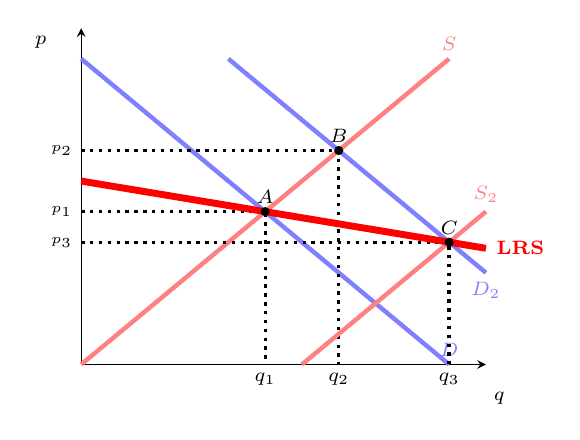
\begin{tikzpicture}\scriptsize  
				\begin{axis}[clip=false,
	scale=0.75,
		xlabel=$q$,
		ylabel=$p$,
		%grid=major,
		legend pos=outer north east,
		axis lines=center,
				enlarge x limits={rel=0.1, upper},
		enlarge y limits={rel=0.1, upper},
		every axis y label/.style={at={(axis description cs:-0.1,1)},anchor=north},
		every axis x label/.style={at={(axis description cs:1,-0.1)},anchor=west},
		ticks=none,
		ymax=10,
		ymin=0,
		]
		\addplot[ultra thick, domain=0:10,red!50, samples=30]{x};
		\addplot[ultra thick, domain=0:10,blue!50]{10-x};
		\draw[ultra thick, blue!50] (axis cs:4,10)--(axis cs:11,3)node[below]{$D_2$};
		\draw[very thick, dotted] (axis cs:0,5)node[left]{\tiny $p_1$}--(axis cs:5,5)--(axis cs:5,0)node[below]{$q_1$};
		\draw[blue!50] (axis cs:10,0)node[above]{$D$};
		\draw[red!50] (axis cs:10,10)node[above]{$S$};
		\draw[very thick, dotted] (axis cs:0,7)node[left]{\tiny $p_2$}--(axis cs:7,7)--(axis cs:7,0)node[below]{$q_2$};
		\draw[ultra thick, red!50] (axis cs:6,0)--(axis cs:11,5)node[above]{$S_2$};
		\draw[very thick, dotted] (axis cs:0,4)node[left]{\tiny $p_3$}--(axis cs:10,4)--(axis cs:10,0)node[below]{$q_3$};
		\draw[line width=2.5, red] (axis cs:0,6)--(axis cs:11,3.8)node[right]{\textbf{LRS}};
		\draw[fill=black] (axis cs:5,5)circle(0.05cm)node[above]{$A$};
		\draw[fill=black] (axis cs:7,7)circle(0.05cm)node[above]{$B$};
		\draw[fill=black] (axis cs:10,4)circle(0.05cm)node[above]{$C$};
		\end{axis} 
 			\end{tikzpicture}\\
		\end{tabular}
	\end{table}
		\begin{itemize}
			\item \textbf{Short run}: $A \rightarrow B$: increase in demand, firms earn profit
			\item \textbf{Long run}: $B \rightarrow C$: profits attract entry
			\begin{itemize}
				\item Entry lowers costs to all firms (dashed curves) 
				\item Entry continues until price falls to $p_3$ (lower than $p_1$), where $p=AC(q)=MC(q)$ and $\pi=0$ for all firms
				\item Long run supply curve is downward sloping due to decreased costs
			\end{itemize} 
		\end{itemize}
	\end{itemize}
\end{itemize}

\clearpage


\end{document}
